\chapter{基于物理过程的侧向流模拟}\label{ch:侧向流模拟}

CoLM中基于流域单元网格,发展了对坡面流、河道径流和地下水侧向流的模拟方案(图~\ref{fig:主要水文过程})。

{
\begin{figure}[htbp]
\centering
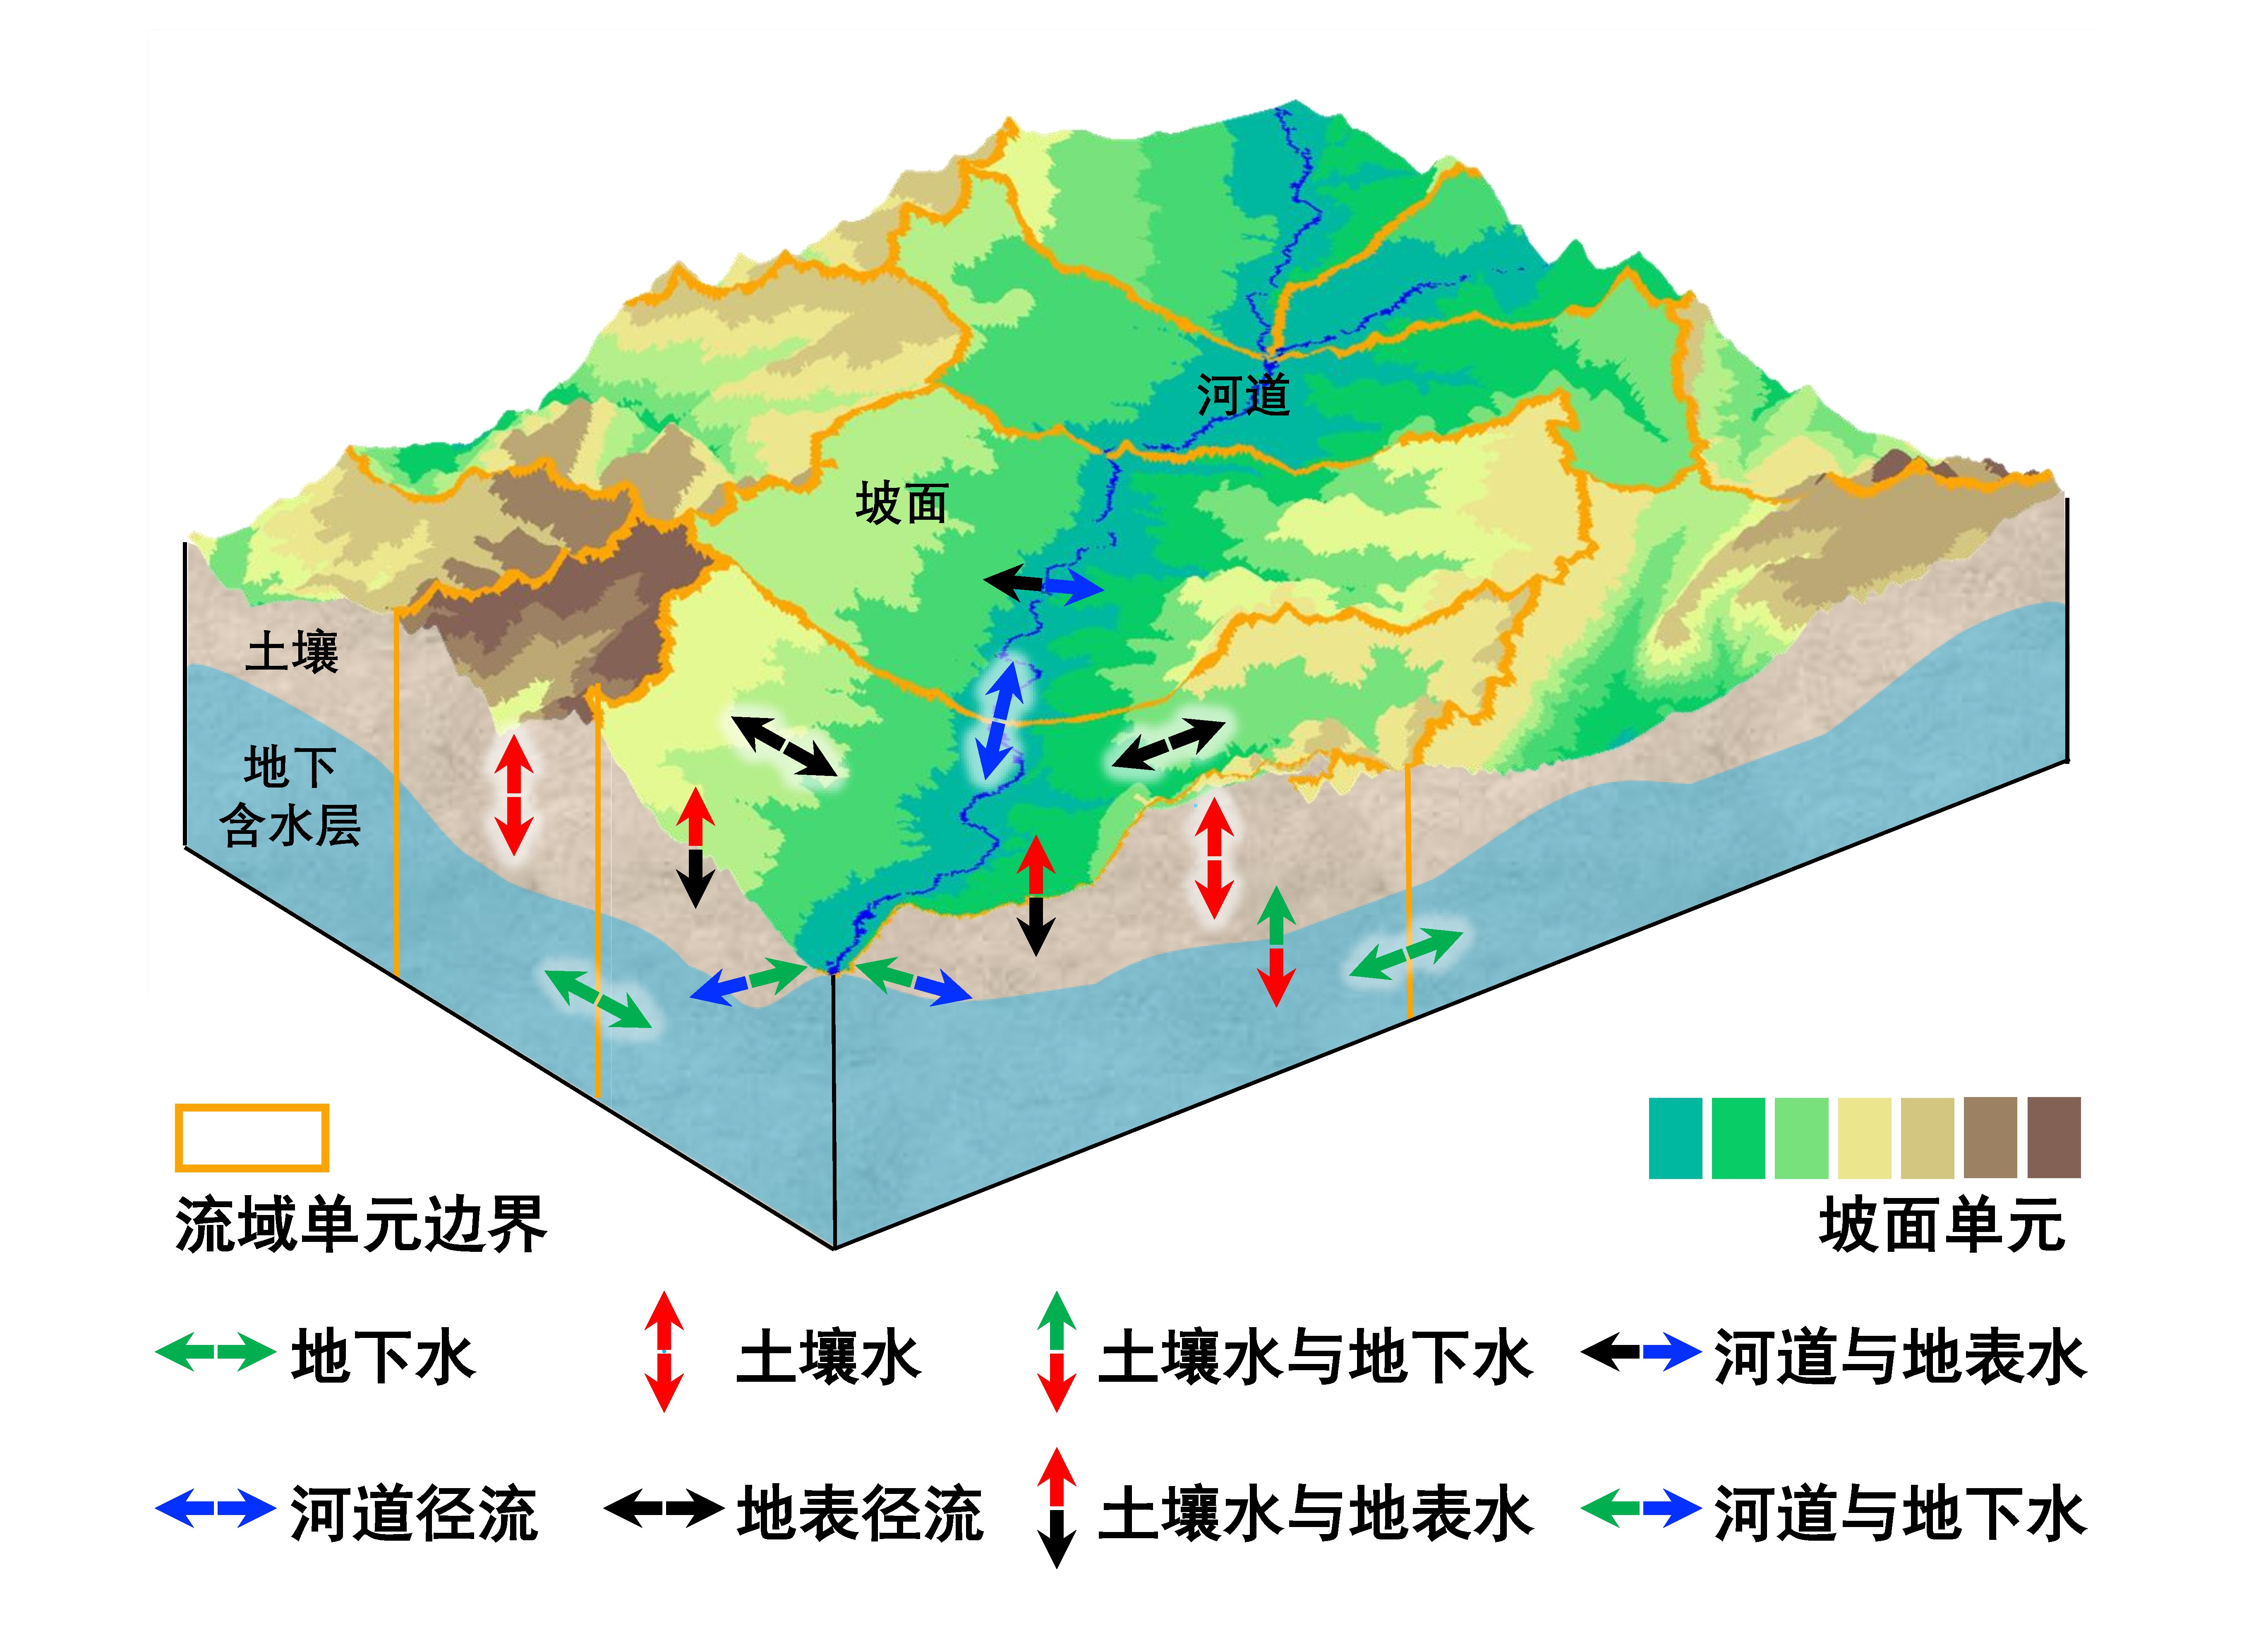
\includegraphics[width=\textwidth]{Figures/侧向流/主要水文过程.jpg}
\caption{基于物理过程的侧向流模拟中的主要水文过程}
\label{fig:主要水文过程}
\end{figure}
}

河道径流发生在流域单元之间。流域单元网格基于集水和汇流关系对模拟区域进行剖分,一个流域单元与一段河道相关联。模式中假设一个流域单元内的水分在地形的主要作用下汇集到河道后,在河道中沿地势而向下流动。

坡面流发生在高度带单元之间,在流域单元内部进行。流域单元内部的高度带都是连通的,且每个高度带具有唯一的下游单元,因此,水流在高度带单元之间的流动路径是清晰的,可基于物理方程进行模拟。通过将河道作为最低处的高度带,CoLM实现了对河道径流和坡面流的相互作用的描述。

地下水的侧向流动包含三个级别:流域单元之间、高度带单元之间以及次网格单元之间。在模拟高度带单元之间的地下水侧向流时,通过将河道作为最低处的单元,实现了对河道径流和地下水侧向流的相互作用的描述。

\section{坡面流、河道径流}

\begin{mymdframed}{代码}
本节对应的代码文件为\texttt{HYDRO/MOD\_Hydro\_HillslopeFlow.F90} \\
和\texttt{HYDRO/MOD\_Hydro\_RiverLakeFlow.F90}.
\end{mymdframed}

{
\begin{figure}[htbp]
\centering
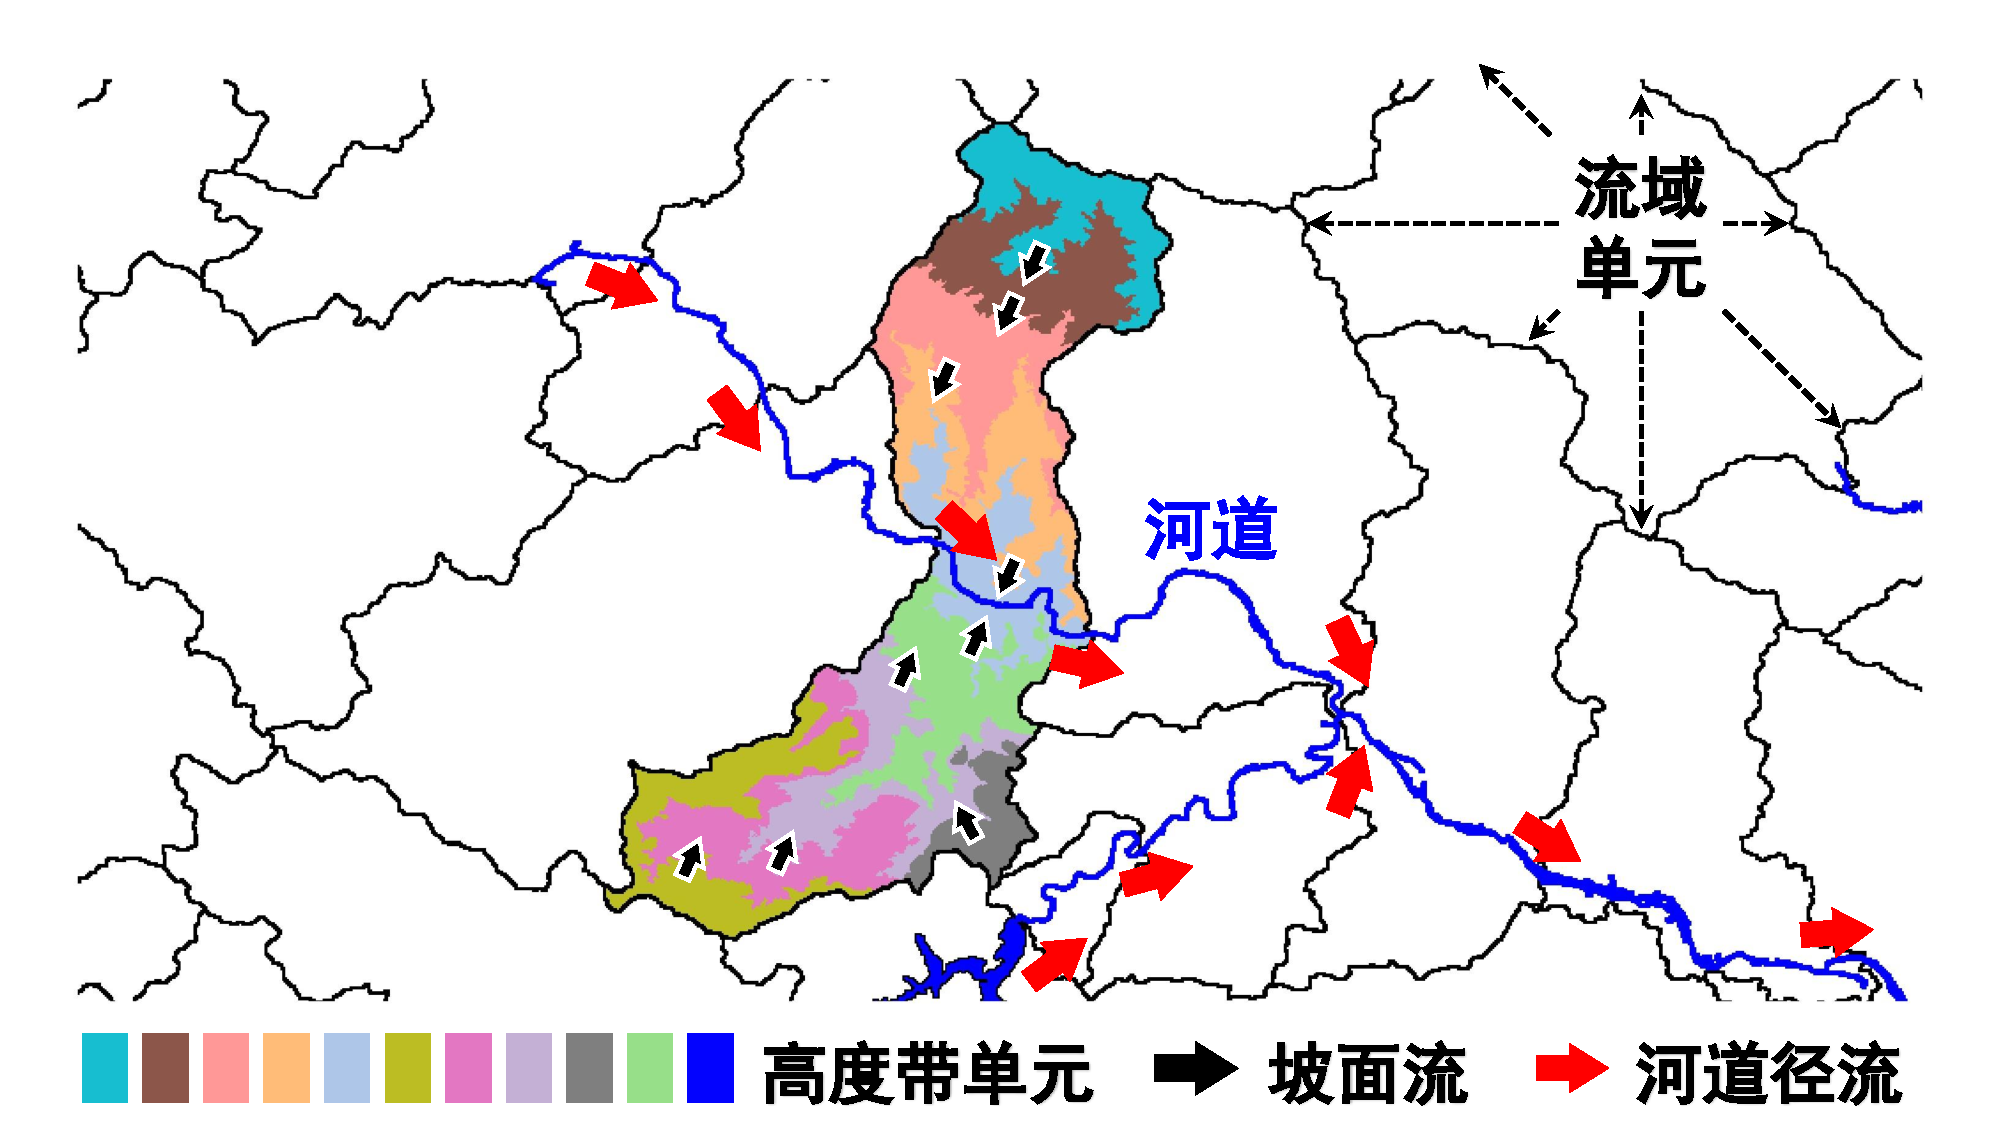
\includegraphics[width=\textwidth]{Figures/侧向流/坡面流和河道径流.pdf}
\caption{CoLM中的坡面流和河道径流}
\label{fig:坡面流和河道径流}
\end{figure}
}

对坡面流和河道径流的模拟基于完整的浅水波方程.
 \subsection{浅水波方程}
 质量方程
  \begin{equation}
 \frac{\partial h}{\partial t} + \frac{\partial \left(uh\right)}{\partial s} = 0
 \end{equation}
 动量方程
 \begin{equation}
 \frac{\partial \left(uh\right)}{\partial t} + \frac{\partial}{\partial s}\left(u^2h+\frac{1}{2}gh^2\right) = -gh\frac{\partial z_b}{\partial s}-gh\frac{n^2\left|q\right|}{h^{10/3}}q
  \end{equation}
  其中,$h$表示水深(单位m),$u$表示水流速度(单位 \unit{m.s^{-1}}),$t$表示时间(单位s),$s$表示沿水流路径的长度(单位m),$q=uh$表示单位宽度的流量(单位 \unit{m^2.s^{-1}}),$z_b$表示坡面的高度(单位m),$n$表示曼宁系数(单位 \unit{m^{-1/3}.s})。


\subsection{数值离散格式}
坡面流是指在一个流域单元内部地表水的流动,它主要描述地表水从集水区域到河道的过程,即产流的过程。CoLM中将一个流域单元划分为多个面积相近的高度带单元,作为计算坡面流的基本离散单元。一般情况下,水流由地势较高的单元流向地势较低的单元,发生洪水时,也可由河道向上淹没地势较高的区域。浅水波方程的预报变量水深$h$和水流速度$u$定义在高度带单元上(图~\ref{fig:坡面流和河道径流})。

河道径流是指流域单元之间地表水的流动,主要沿河道进行。CoLM基于水文学数据划分流域单元,与流域单元关联的分段河道之间有明确的上下游关系,为计算河道径流的基本离散单元。一般情况下,水流由地势较高的河道流向地势较低的河道,可经过湖泊或者水库,最后汇流入海,或者终止于内陆洼地。浅水波方程的预报变量水深$h$和水流速度$u$定义在分段河道上(图~\ref{fig:坡面流和河道径流})。

{
\begin{figure}[htbp]
\centering
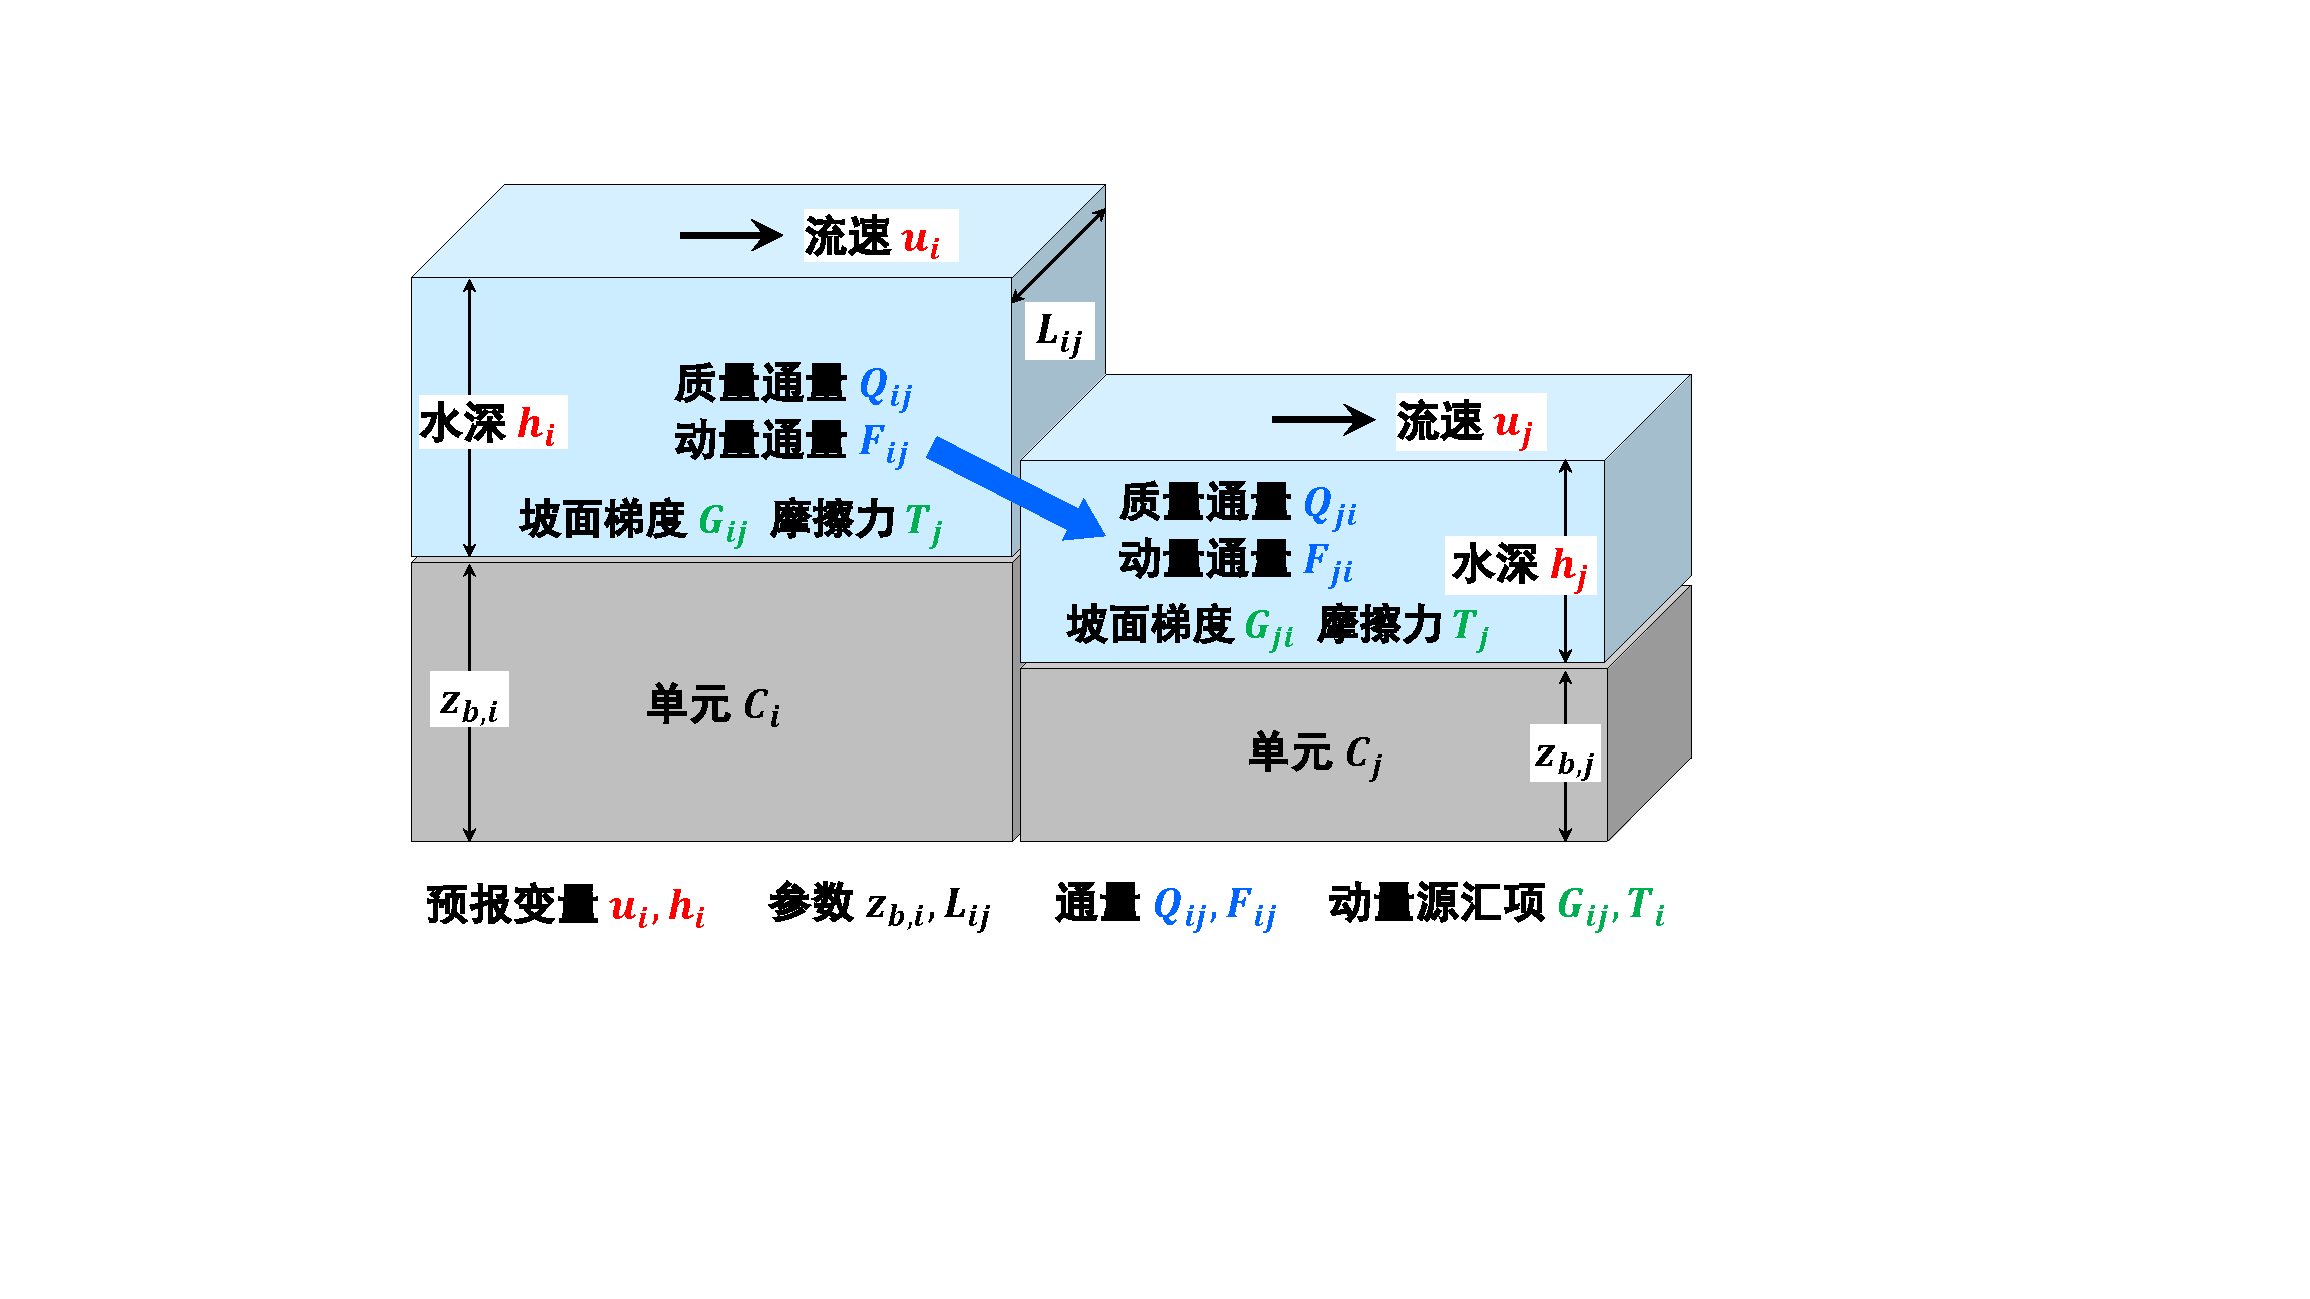
\includegraphics[width=0.8\textwidth]{Figures/侧向流/浅水波方程求解.pdf}
\caption{浅水波方程求解方案中的变量}
\label{fig:浅水波方程求解}
\end{figure}
}

 质量方程离散为
  \begin{equation} \label{formula:mass_swe}
 \frac{ h^{n+1}_i - h^n_i}{\Delta t} A_i+\sum_{j\in K_i} Q^n_{ij} = 0
 \end{equation}
 动量方程离散为
 \begin{equation}
 \frac{ \left(uh\right)^{n+1}_i - \left(uh\right)^n_i}{\Delta t} A_i + \sum_{j\in K_i} F^n_{ij} = \sum_{j\in K_i} G^n_{ij}  + T^{n+1}_i  A_i \label{swe-d-2}
  \end{equation}
其中(图~\ref{fig:浅水波方程求解}),
\begin{itemize}
\item $n$和$n+1$表示时间步数,时间步长为$\Delta t$;
\item $C_i$表示标号为$i$的空间单元,$A_i$表示$C_i$的面积;
\item $K_i$表示与$C_i$有水分交换的其余空间单元的标号的集合;
\item $Q_{ij}$表示从$C_i$到$C_j$的质量通量,$F_{ij}$表示从$C_i$到$C_j$的动量通量;
\item $G_{ij}$表示$C_i$与$C_j$之间由坡面梯度形成的动量的源汇项;
\item $T_i$表示$C_i$上坡面的摩擦力。
\end{itemize}

假设两个相邻的水文单元为$C_i$和$C_j$,其中$C_i$为上游单元,$C_j$为下游单元。离散格式中各项的计算方法如下:

{
\begin{figure}[htbp]
\centering
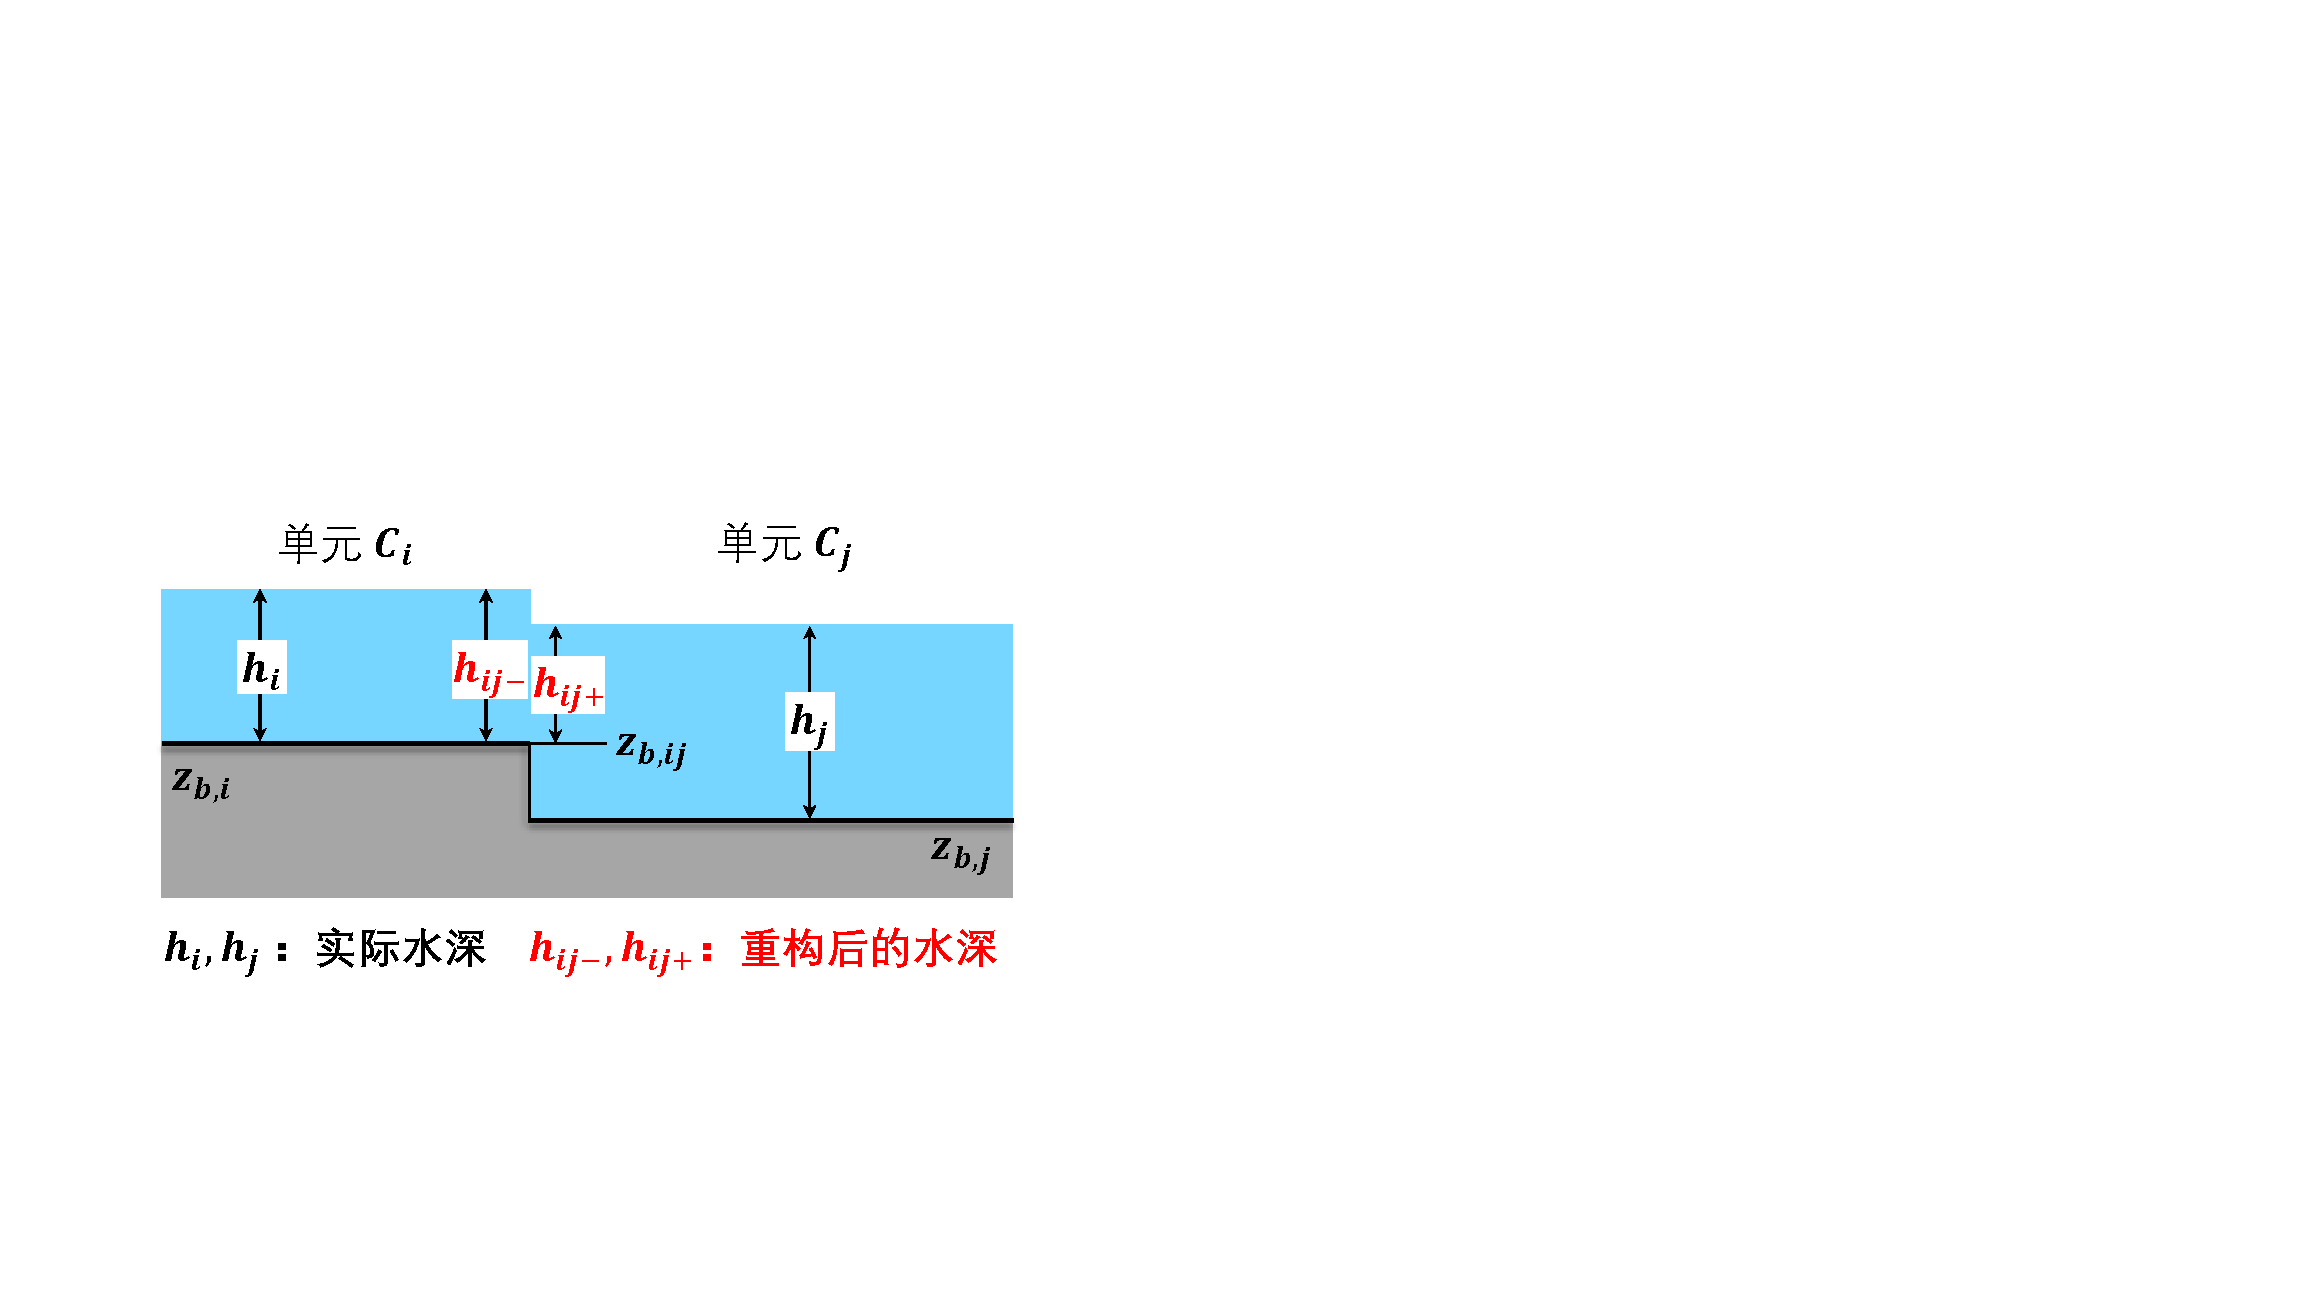
\includegraphics[width=0.6\textwidth]{Figures/侧向流/水深重构.pdf}
\caption{浅水波方程求解方案中对水深的重构(公式见~\ref{formula:water_depth_reconstruction})}
\label{fig:水深重构}
\end{figure}
}

(1)首先对边界上的$h$进行重构~\citep{audusse2004scientificcomputing}(见图~\ref{fig:水深重构}),
\begin{equation} \label{formula:water_depth_reconstruction}
\begin{aligned}
z_{b,ij} & = \max\left(z_{b,i}, z_{b,j}\right) \\
h_{ij-} & =  \max\left(0, h_i + z_{b,i} - z_{b,ij} \right) \\
h_{ij+} & =  \max\left(0, h_j + z_{b,j} - z_{b,ij} \right)
\end{aligned}
\end{equation}
其中$h_{ij-}$表示界面处$C_i$一侧的重构值,$h_{ij+}$表示界面处$C_j$一侧的重构值。

(2)局部黎曼问题中,中间区域的速度$u_{ij*}$计算为
	\begin{equation}
		u_{ij*} = \frac{1}{2}\left(u_i + u_j\right) + \sqrt{g h_{ij-}} - \sqrt{g h_{ij+}}
	\end{equation}
其中,$u_i$和$u_j$分别为$C_i$和$C_j$中的水流的速度。 

局部黎曼问题中,中间区域的水深$h_{ij*}$计算为
	\begin{equation}
		h_{ij*} = \frac{1}{g}\left[\frac{1}{2}\left(\sqrt{g h_{ij-}} + \sqrt{g h_{ij+}}\right) + \frac{1}{4}\left(u_i - u_j\right)\right]^2
	\end{equation}

(3)上游波速$S_{ij-}$计算为
	\begin{equation}
		S_{ij-} = \left\{
		\begin{aligned}
			&u_j - 2\sqrt{gh_{ij+}}, && \mbox{if} \quad h_{ij-} = 0 \\
			& \min \left(u_i - \sqrt{gh_{ij-}}, u_{ij*} - \sqrt{gh_{ij*}}\right), && \mbox{if} \quad h_{ij-} > 0
		\end{aligned}\right.
	\end{equation}
下游波速$S_{ij+}$计算为
	\begin{equation}
		S_{ij+} = \left\{
		\begin{aligned}
			&u_i + 2\sqrt{gh_{ij-}}, && \mbox{if} \quad h_{ij+} = 0 \\
			& \max \left(u_j + \sqrt{gh_{ij+}}, u_{ij*} + \sqrt{gh_{ij*}}\right), && \mbox{if} \quad h_{ij+} > 0
		\end{aligned}\right.
	\end{equation}

(4)边界上的通量计算为
\begin{equation}
	Q_{ij} = L_{ij} \cdot \left\{
	\begin{aligned}
		& Q_{ij-}, && \mbox{if} \quad 0\leqslant S_{ij-} \\
		& \frac{S_{ij+} Q_{ij-} - S_{ij-} Q_{ij+} + S_{ij-} S_{ij+} \left(h_{ij+} - h_{ij-}\right)}{S_{ij+}-S_{ij-}} , && \mbox{if} \quad S_{ij-} \leqslant 0\leqslant S_j\\
		& Q_{ij+}, && \mbox{if} \quad 0\geqslant S_{ij+}
	\end{aligned}\right.
\end{equation}

\begin{equation}
F_{ij} = L_{ij} \cdot 
\begin{cases}
	 F_{ij-}, & \mbox{if} \quad 0\leqslant S_{ij-} \\
	 \frac{S_{ij+} F_{ij-} - S_{ij-} F_{ij+} + S_{ij-} S_{ij+} \left(q_{ij+} - q_{ij-}\right)}{S_{ij+}-S_{ij-}} , & \mbox{if} \quad S_{ij-} \leqslant 0\leqslant S_{ij+}\\
	F_{ij+}, & \mbox{if} \quad 0\geqslant S_{ij+}
\end{cases}
\end{equation}
其中,$L_{ij}$为单元$C_i$与$C_j$之间交界线的长度,边界两侧的重构量
\begin{align*}
&Q_{ij-} = q_{ij-} = u_i h_{ij-},  && Q_{ij+} = q_{ij+} = u_j h_{ij+}, \\
&F_{ij-} = u_i^2h_{ij-}+\frac{1}{2}gh_{ij-}^2, && F_{ij+} = u_j^2h_{ij+}+\frac{1}{2}gh_{ij+}^2
\end{align*}

(5)由坡面梯度形成的动量的源汇项计算为~\citep{audusse2004scientificcomputing}
\begin{equation}
G_{ij} = \frac{1}{2}gh_{ij-}^2 \cdot L_{ij}, \quad
G_{ji}=-\frac{1}{2}g h_{ij+}^2 \cdot L_{ij}
\end{equation}
注意,$G_{ji}$不出现在$C_i$单元的离散动量方程(\ref{swe-d-2})中,而是在$C_j$单元的离散动量方程中使用. 因为不是通量项,所以$G_{ij}$与$G_{ji}$不一定互为相反数。

通量项满足$Q_{ji} = -Q_{ji}$,$F_{ji}=-F_{ji}$.

(6)摩擦力项采用半隐离散格式
\begin{equation}
T^{n+1}_i = -g \left(\frac{n^2}{h^{7/3}} \left|q\right|\right)^n_i q^{n+1}_i
\end{equation}
代入离散后的动量方程可得,
 \begin{equation}
 \frac{ q^{n+1}_i - q^n_i}{\Delta t} A_i + \sum_{j\in K_i} F^n_{ij} = \sum_{j\in K_i} G^n_{ij}  -g \left(\frac{n^2}{h^{7/3}} \left|q\right|\right)^n_i q^{n+1}_i  A_i 
  \end{equation}

综合起来,单宽流量的更新采用下列格式
\begin{equation}
q^{n+1}_i = \frac{q^n_i - \frac{\Delta t}{A_i}\sum_{j\in K_i} \left(F^n_{ij} - G^n_{ij}\right)}{1 + g \left(\frac{n^2}{h^{7/3}} \left|q\right|\right)^n_i \Delta t}
\end{equation}

\subsection{自适应时间步长方法}
对时间步长的约束包含三个,$\Delta t = \min \Delta t_i \quad (i=1, \ldots, N)$,
\begin{enumerate}
\item CFL条件
\begin{equation}
\qquad \Delta t_i \leqslant \mathrm{C}\frac{ D_i }{\left| u_{i}\right| + \sqrt{gh_{i}}}
\end{equation}
其中,$D_i$为第$i$个单元的平均水流路径长度,C为Courant数,模式里取值为0.8。
\item 质量限制:
当$\sum_{j\in K_i} Q_{ij}>0$时,
  \begin{equation}
 \Delta t_i \leqslant \frac{h^n_i\cdot A_i}{\sum_{j\in K_i} Q_{ij}}
 \end{equation}
\item 动量限制:
当$q^n_i \cdot \left[ \frac{1}{A_i}\sum_{j\in K_i} \left(F^n_{ij} - G^n_{ij} \right)\right] > 0$ 且 $\mathrm{abs}\left(q^n_i\right) > q_{min}$时,
  \begin{equation}
 \Delta t_i \leqslant \frac{q^n_i}{\frac{1}{A_i}\sum_{j\in K_i} \left(F^n_{ij} - G^n_{ij} \right)}
 \end{equation}
其含义为在一个时间步长内,速度不改变方向。
 \end{enumerate}

\subsection{数值算法在模式中的实现}

\subsubsection{参数的计算}
离散算法中需要的参数有平均水流路径的长度$D_i$,两个单元的边界线的长度$L_{ij}$,单元的面积$A_i$和单元表面的高度$z_{b,i}$,以及曼宁系数$n$.

对高度带单元:1)单元面积$A_i$指土壤、城市和湿地面积的总和(排除冰川和水体);2)单元表面的高度$z_{b,i}$定义为排水高度(一个像素点和它流入的河道点的高度差Height Above Nearest Drainage, HAND);3)长度$L_{ij}$为两个单元的边界线的长度;4)单元内一个像素点的水流路径定义为:自这个像素点开始,沿水流方向直至离开这个单元前的最后一个像素点之间的距离;平均水流路径定义为所有像素点的水流路径的算术平均值;5)曼宁系数$n$取常数$0.3$。

对分段河道:1)单元面积$A_i$指河道的面积;2)单元表面的高度$z_{b,i}$定义为河床的高度;3)长度$L_{ij}$为相邻两段河道的宽度的算术平均值,河道的宽度使用河道的面积除以河道的长度计算得到;4)平均水流路径$D_i$为河道的长度;5)曼宁系数$n$取常数$0.03$。

河道深度根据集水区域上的产流量进行估算,采用CaMa-Flood~(v4)~\citep{yamazaki2011physically}中的经验公式,
\begin{equation}
B = \max \left[0.1\times R_{\mathrm{up}}^{0.5}, 1.00\right]
\end{equation}
其中,$R_{\mathrm{up}}$为河道上游集水区域的平均产流速度(\unit{m^3.s^{-1}})。

\subsubsection{洪泛过程} \label{sec:lateral_flood}

{
\begin{figure}[htbp]
\centering
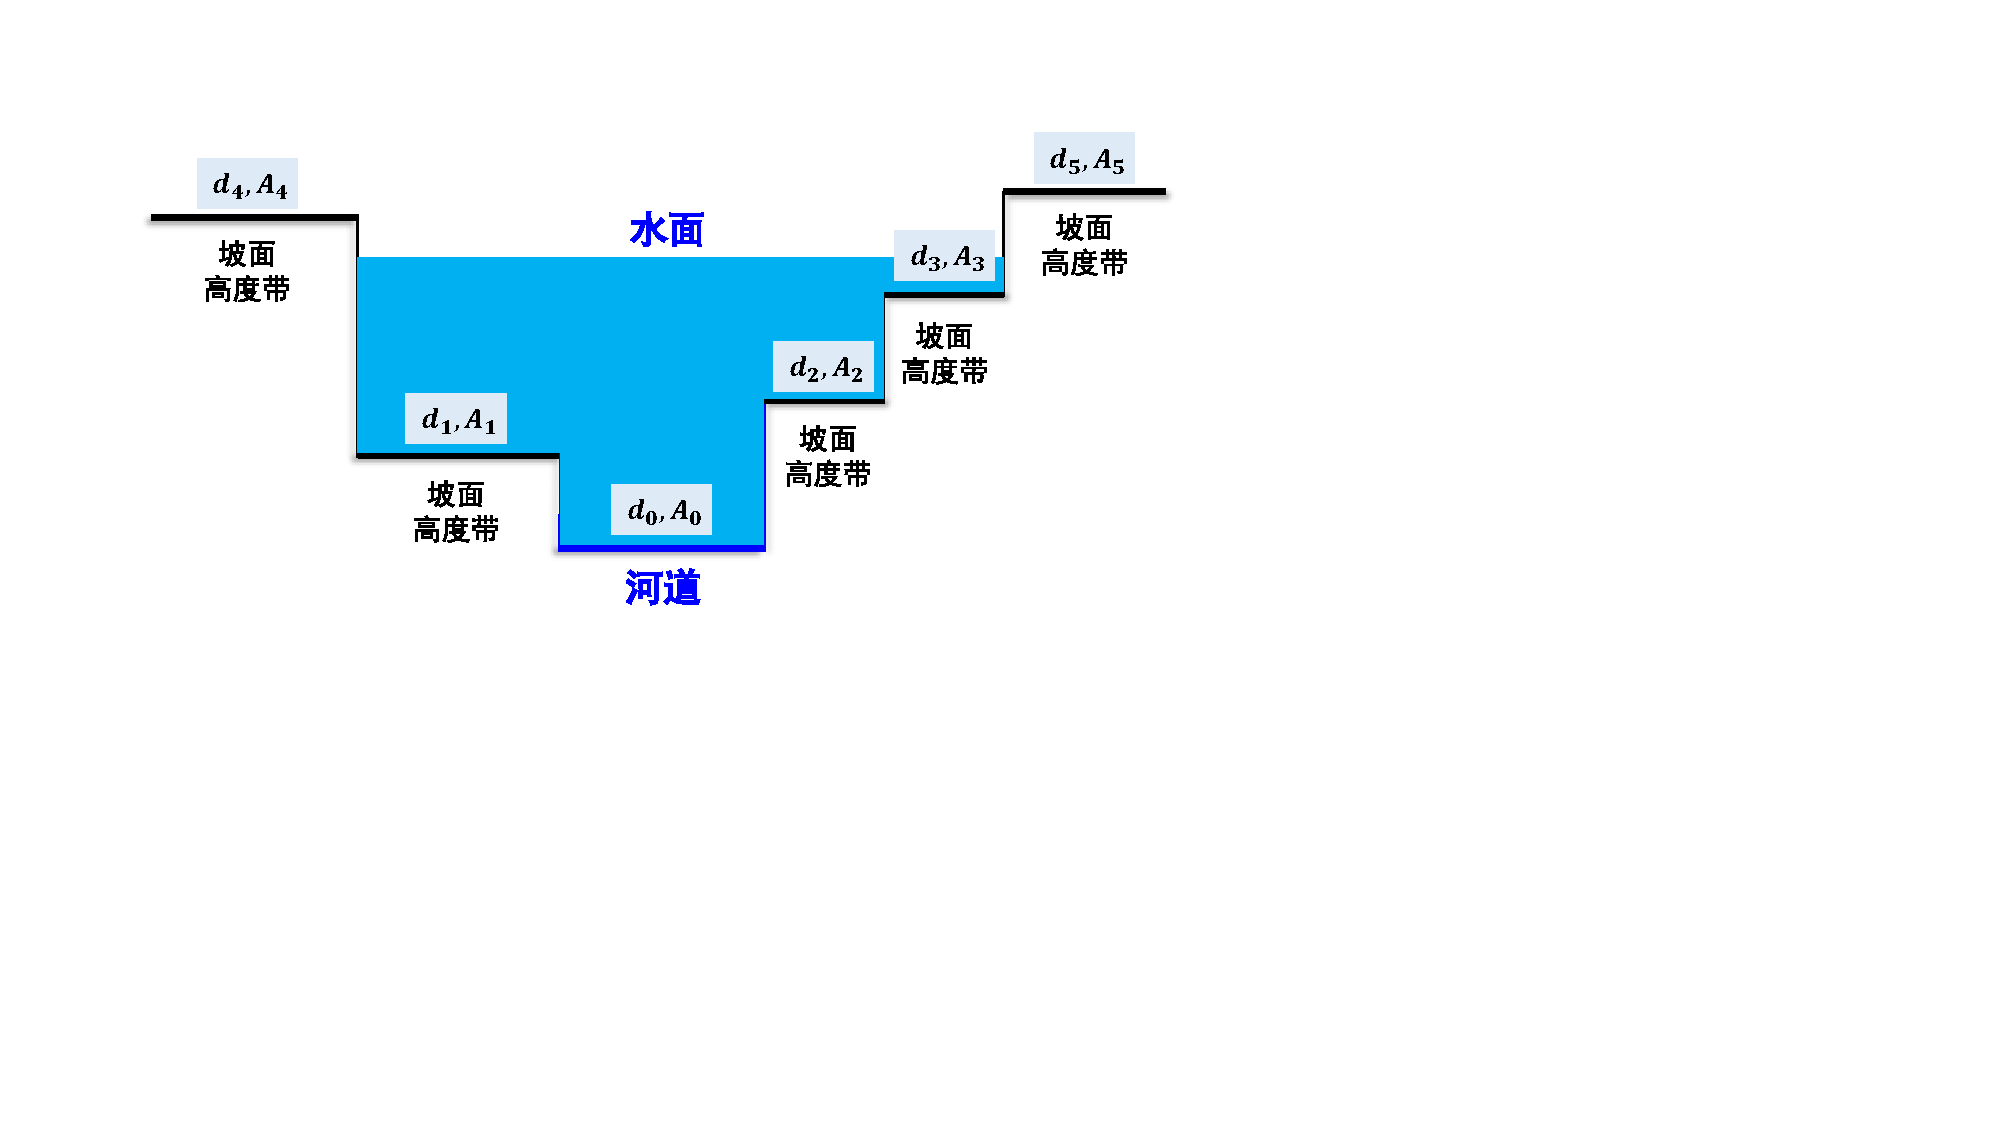
\includegraphics[width=0.8\textwidth]{Figures/侧向流/发生洪泛时的水深.pdf}
\caption{发生洪泛的水深示意图}
\label{fig:lateral_flood}
\end{figure}
}
在河道径流的模拟中,当河道中的水深超过河道深度时,即发生洪泛事件。模式中不考虑发生洪泛事件时河道与高度带单元之间的水动力过程,因此,由预报方程~\eqref{formula:mass_swe}得到总水量$V^{n+1}_i$后,超出河道深度的水量按照从低到高的顺序分配到高度带单元上~(图~\ref{fig:lateral_flood})。假设由低到高的高度带单元(河道为最低的单元)的面积和高度分别为$A_{0},A_{1},\ldots,A_{J}$和$d_{0},d_{1},\ldots,d_{J}$,则从总水量$V$到水深$h$的分段函数定义为
\begin{equation}
    h(V) = \begin{cases}
			\frac{V}{A_0}, & V \leqslant A_{0} \left(d_1 - d_0\right)\\
            \frac{V-A_{0} \left(d_1 - d_0\right)}{A_0+A_1}, & A_{0} \left(d_1 - d_0\right) < V \leqslant A_{0} \left(d_2 - d_0\right) + A_{1} \left(d_2 - d_1\right) \\
            \cdots, & \cdots \\
            \frac{V-\sum^{j-1}_{k=0}A_k(d_{j}-d_k)}{\sum^j_{k=0}A_k}, & \sum^{j-1}_{k=0}A_k(d_{j}-d_k) < V \leqslant \sum^{j}_{k=0}A_k(d_{j+1}-d_k)\\
            \cdots, & \cdots  \\
            \frac{V-\sum^{J-1}_{k=0}A_k(d_{J}-d_k)}{\sum^J_{k=0}A_k}, & \sum^{J-1}_{k=0}A_k(d_{J}-d_k) < V 
		 \end{cases}
\end{equation}

总水量$V$和水深$h$之间的映射为一一映射,由水深也可计算得到总水量。模式中计算河道径流时,水深定义为流域单元内最低的水面位置到河道底部的距离。

\subsubsection{湖泊单元}
湖泊的水量变化与与河道径流一起进行计算。在模式中,一个完整的湖泊(边界来自于HydroLAKES数据)设置为一个湖泊单元,因此,其面积不受流域单元面积阈值的限制。对面积较大的湖泊单元,将其进一步划分为多个小单元(划分方法见图~\ref{fig:湖泊划分})。使用高精度的湖泊深度数据,可聚合得到这些小单元上的平均深度,根据小单元的面积和深度可建立总水量和水深的函数映射(方法同\ref{sec:lateral_flood})。对湖泊单元,始终使用总水量和水深的函数映射,湖泊中的水深和总水量的更新步骤为:1)使用水深计算湖泊单元与邻居单元之间的水流通量;2)使用水流通量计算变化后的总水量;3)根据更新后的总水量,使用函数映射计算新的水深。对流域单元,只在发生洪泛事件时使用总水量和水深的函数映射。

目前模式中未考虑湖泊水体的动量的变化。

\section{地下水侧向流}

\begin{mymdframed}{代码}
本节对应的代码文件为\texttt{HYDRO/MOD\_Hydro\_SubsurfaceFlow.F90}.
\end{mymdframed}

CoLM中计算三个等级上的单元之间的地下水侧向流:流域单元之间、高度带单元之间以及次网格单元之间(图~\ref{fig:地下水侧向流})。模型基于坡面蓄水型Boussinesq方程。

{
\begin{figure}[htbp]
\centering
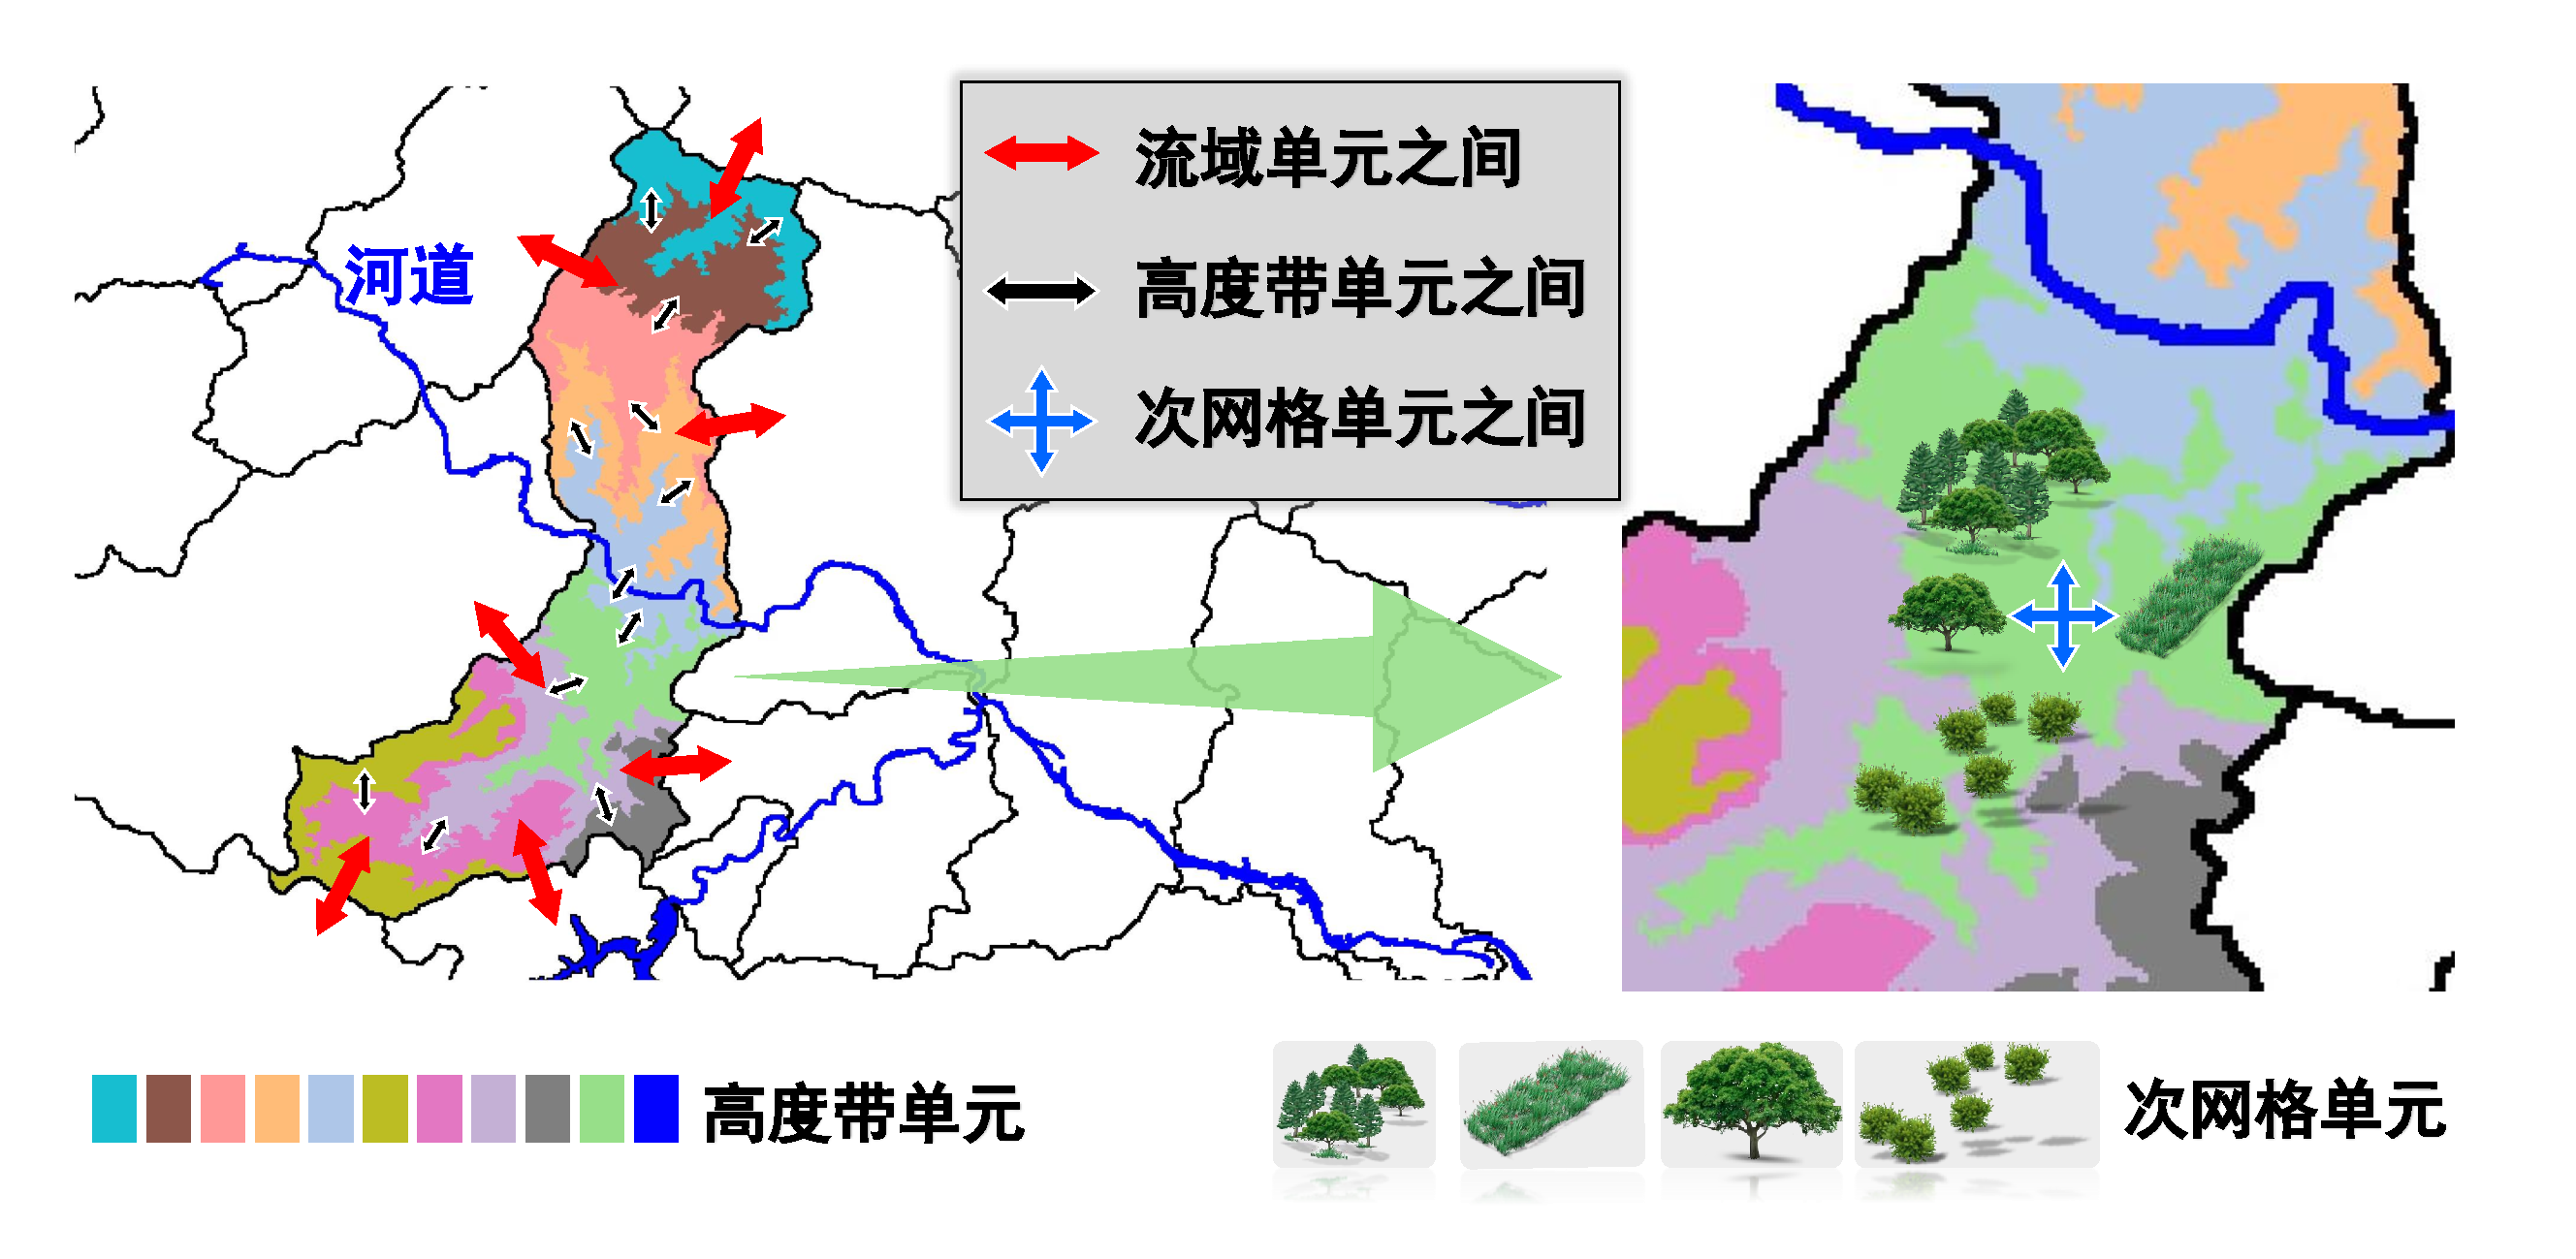
\includegraphics[width=\textwidth]{Figures/侧向流/地下水侧向流.pdf}
\caption{CoLM中的地下水侧向流}
\label{fig:地下水侧向流}
\end{figure}
}

\subsection{方程及数值算法}
\subsubsection{坡面蓄水型Boussinesq方程}
坡面蓄水型Boussinesq方程为
\begin{equation}
\frac{\partial \left(fh\right)}{\partial t} = \frac{\partial}{\partial x} \left[\cos i \cdot \left(kh\frac{\partial h}{\partial x}\right)+\sin i\cdot k\frac{\partial h}{\partial x}\right]
\end{equation}
其中,$h$表示饱和水层在垂直于不透水面方向上的厚度(单位m);$t$表示时间(单位s);$x$表示沿不透水面向上的方向(单位m);$i$表示不透水面的倾斜角;$k$表示水力导度(单位 \unit{m.s^{-1}});$f$表示可排水的孔隙度(单位 \unit{m.m^{-1}}).

\subsubsection{方程的简化}
假设垂直于不透水面的方向为$y$方向(从地表向下为正方向),土壤厚度为$H$,当$k$在$y$方向有变化时,$kh$替换为$y$方向的积分
\begin{equation}
\int^H_{H-h} k \  \mathrm{d}y
\end{equation}
记地下水位为$z_{wt}=H-h$,代入可得
\begin{equation}
\frac{\partial \left(fz_{wt}\right)}{\partial t} = \frac{\partial}{\partial x} \left[ \cos i \cdot \left(\int^{H}_{z_{wt}} k \mathrm{d}y\right)\frac{\partial z_{wt}}{\partial x} +\sin i\cdot k\frac{\partial z_{wt}}{\partial x}\right]
\end{equation}
当不考虑不透水面(基岩)时,可令$H\to \infty$,$i=0$,则方程变为
\begin{equation}
\frac{\partial \left(fz_{wt}\right)}{\partial t} = \frac{\partial}{\partial x} \left[ \left(\int^\infty_{z_{wt}} k\ \mathrm{d}z\right)\frac{\partial z_{wt}}{\partial x} \right]
\end{equation}

\subsubsection{通量的计算:相邻单元之间的半隐格式}
假设相邻水文单元之间交界面的宽度为$w$,则它们之间的水流通量为
$$q=-w\cdot \left(\int^\infty_{z_{wt}} k\ \mathrm{d}z\right)\frac{\partial z_{wt}}{\partial x} $$
水分只在两个单元$C_i$和$C_j$($x$由$C_i$指向$C_j$)之间交换时,方程可离散为
\begin{eqnarray}
z_{wt,i}^{n+1} &=& z_{wt,i}^{n} - \frac{\Delta t}{g_i}\left[ -  w k^n_{ij} \frac{z_{wt,j}^{n+1} - z_{wt,i}^{n+1}}{d_i+d_j} \right], \\
z_{wt,j}^{n+1} &=& z_{wt,j}^{n} + \frac{\Delta t}{g_j}\left[ -  w k^n_{ij} \frac{z_{wt,j}^{n+1} - z_{wt,i}^{n+1}}{d_i+d_j} \right]
\end{eqnarray}
其中,$k^n_{ij}$为界面处的导水率,$g_i=f_iA_i,g_j=f_jA_j$为孔隙度和面积之积。

由此可解出
\begin{eqnarray}
z_{wt,i}^{n+1} &=& \frac{g_i\left(g_j+\sigma\right)z_{wt,i}^{n} +g_j\sigma z_{wt,j}^{n}}{g_ig_j+\left(g_i+g_j\right)\sigma},\\
z_{wt,j}^{n+1} &=& \frac{g_i\sigma z_{wt,i}^{n} +g_j\left(g_i+\sigma\right)z_{wt,j}^{n}}{g_ig_j+\left(g_i+g_j\right)\sigma}\quad \\
\sigma &=& \frac{\Delta t wk_{ij}^n}{d_i+d_j}
\end{eqnarray}
从而水流通量为
\begin{equation}\label{formula:subsurface_lateral_flow}
q = \frac{\sigma}{\Delta t} \frac{g_ig_j}{g_ig_j+\left(g_i+g_j\right)\sigma} \left( z_{wt,i}^{n} - z_{wt,j}^{n} \right)
\end{equation}

公式~\eqref{formula:subsurface_lateral_flow}应用于流域单元之间和高度带单元之间的地下水侧向流计算中。对$C_i$与所有相邻单元之间的水流通量进行叠加,即可得到$C_i$单元上的地下水总量的变化。

\subsubsection{参数的计算}
\begin{itemize}
\item 导水率的计算(来自TOPMODEL)
\begin{equation}
k(z) = K_0\exp{(- z/b)},\quad \int^\infty_{z_{wt}} k\ \mathrm{d}z = b K_0\exp{(-z_{wt}/b)}
\end{equation}
\end{itemize}

\subsubsection{次网格单元之间的地下水交换}
第$i$个高度带单元内部第$p$个patch的地下水侧向流通量为
\begin{equation}
q^{\mathrm{I}}_{i,p} = b K_0 \exp{(-z_{wt,i}/b)}\cdot\frac{z_{wt,i,p}-z_{wt,i}}{\sqrt{A_i/\pi}}
\end{equation}
其中
$$z_{wt,i} = \sum^P_{p=1} \alpha_p z_{wt,i,p}$$
$\alpha_p$为第$p$个patch在整个单元占据的面积比。

不难验证
$$\sum^P_{p=1} \alpha_p q^{\mathrm{I}}_{i,p} =0$$
即$q^{\mathrm{I}}_{i,p}$表达了高度带单元内部的地下水交换。

地下水位和土壤水的变化最终在次网格单元上计算。模式中假设,由流域单元之间的地下水侧向流引起的地下水量的变化在流域单元内部是均匀的,由高度带单元之间的地下水侧向流引起的地下水量的变化在高度带单元内部也是均匀的。因此,在次网格单元上,地下水的总变化量为三个等级的单元上的变化量之和(图~\ref{fig:地下水侧向流})。

由地下侧向流引起的土壤水和地下水的变化计算方案同~\ref{sec:change_of_zwt_vsf}节。

% 若次网格单元上地下水量是减少的($\Delta W < 0$),模式中采用“预估-调整”的方式逐层减少土壤水,降低地下水位。图~\ref{fig:地下水变化}显示了在第$i$层内对地下水位和土壤水的计算方法。

% {
% \begin{figure}[htbp]
% \centering
% 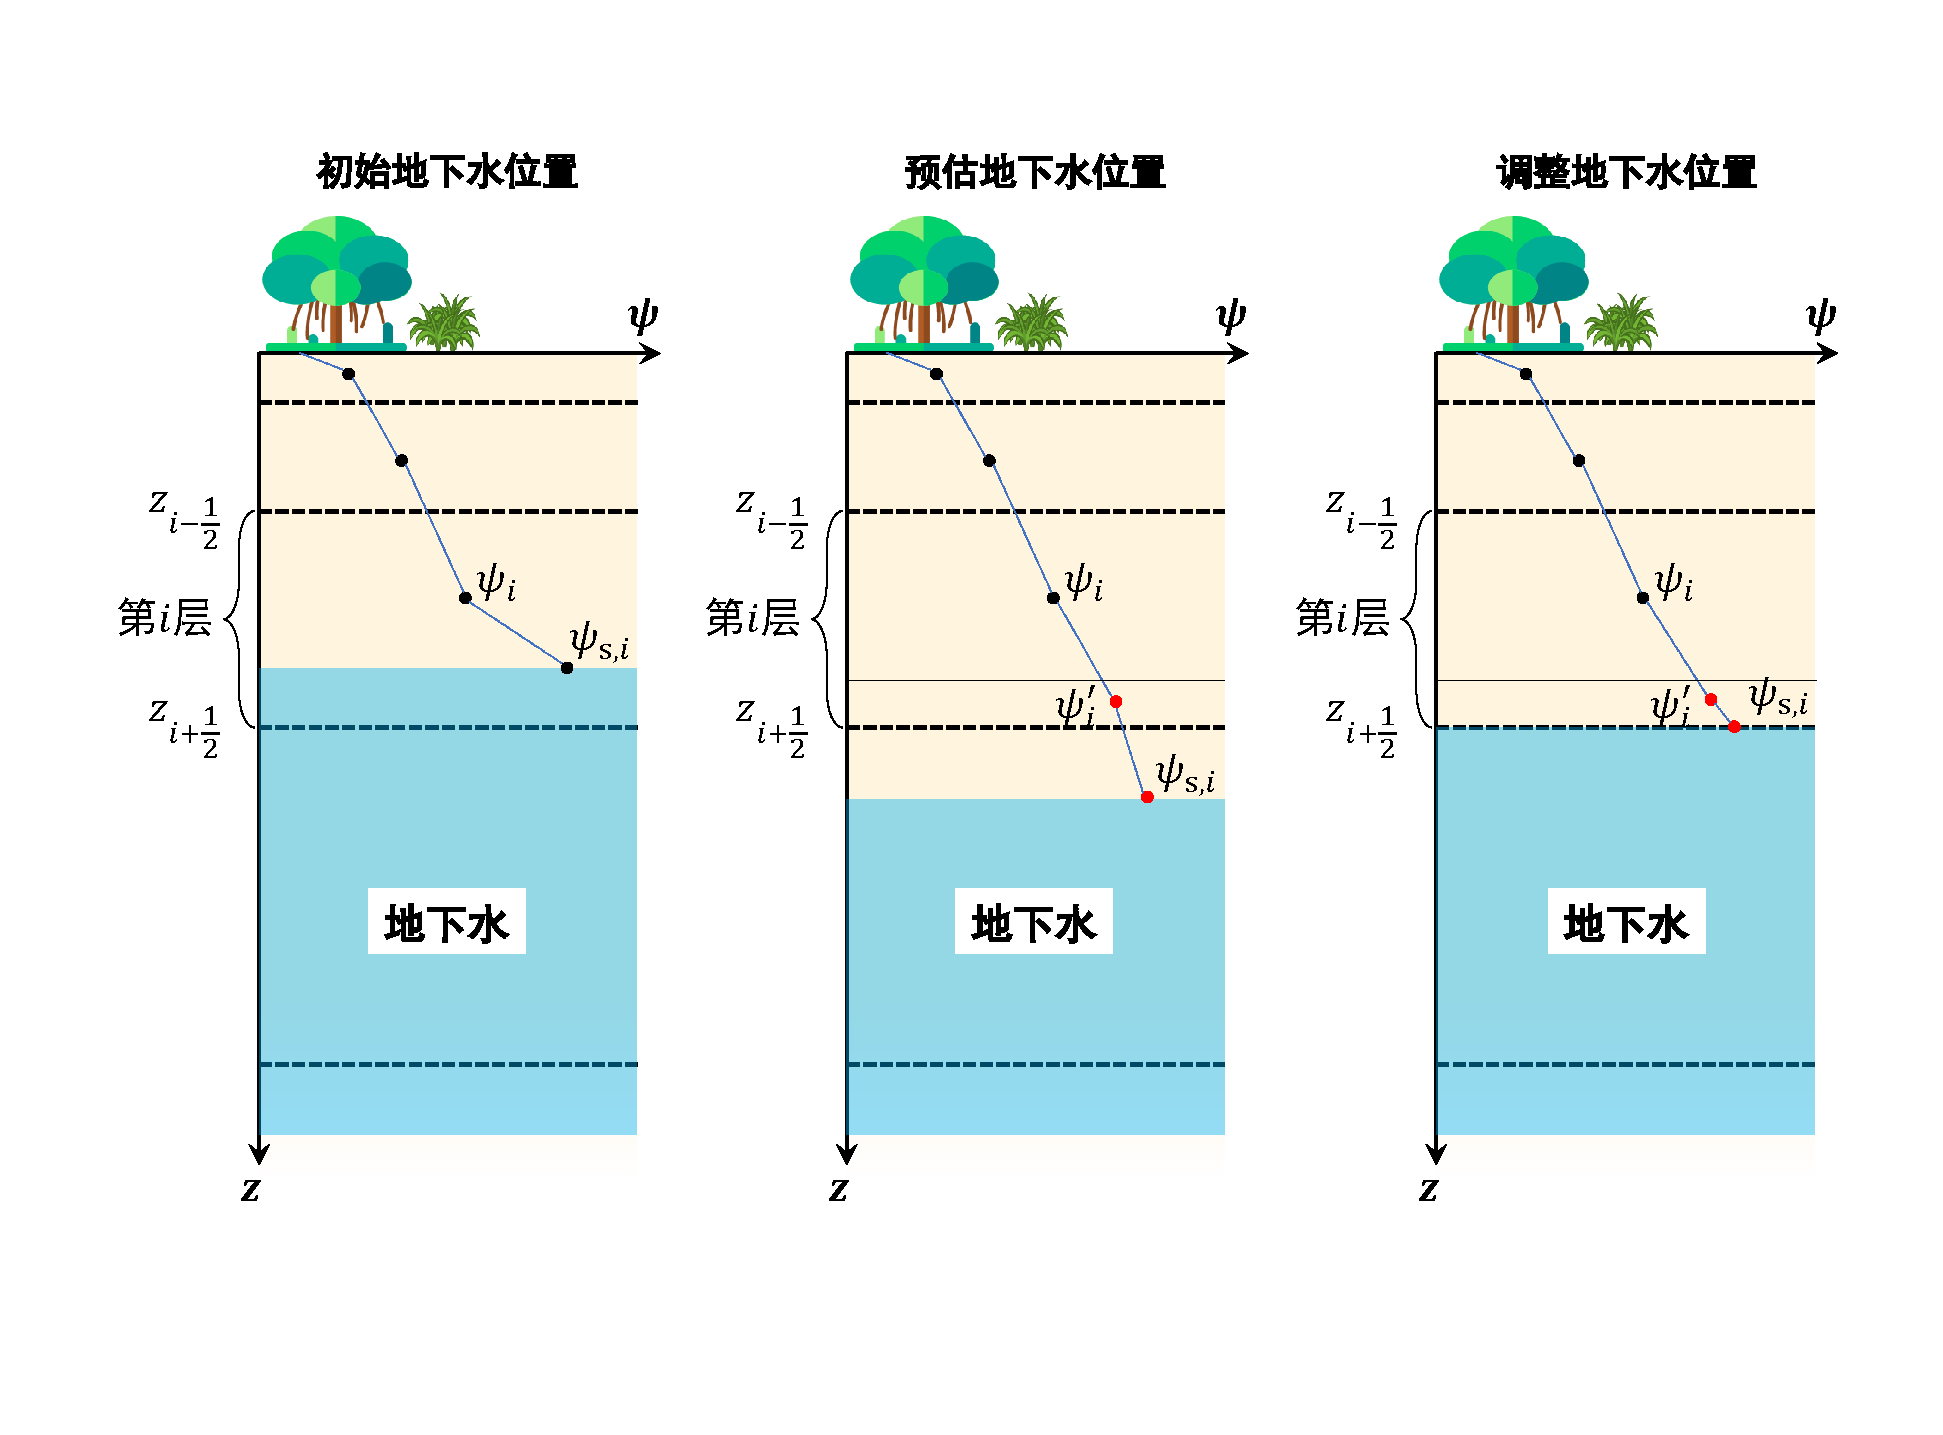
\includegraphics[width=\textwidth]{Figures/侧向流/地下水变化.pdf}
% \caption{地下水减少时地下水位及土壤水变化的计算方案示意图}
% \label{fig:地下水变化}
% \end{figure}
% }

% 在“预估”步,根据目前的地下水位及需减少的水量,预估降低后的地下水位,其满足
% \begin{equation} \label{formula:prediction_zwt}
% \begin{aligned}
% \theta_{\mathrm{pre}} & = \Theta_i\left(\psi_{\mathrm{s},i} - 0.5\left(z_{\mathrm{wt}}^{\mathrm{new}} - z_{\mathrm{wt}}^{\mathrm{old}}\right)\right) \\
%     - \Delta W & = \left(z_{\mathrm{wt}}^{\mathrm{new}} - z_{\mathrm{wt}}^{\mathrm{old}}\right) \times  \left(\theta_{\mathrm{s},i} - \theta_{\mathrm{pre}}\right)
% \end{aligned}
% \end{equation}
% 其中,$z_{\mathrm{wt}}^{\mathrm{old}}$为目前的地下水位,$z_{\mathrm{wt}}^{\mathrm{new}}$为预估的地下水位,$\theta_{\mathrm{s},i}$为饱和含水量,$\psi_{\mathrm{s},i}$为饱和时的土壤水势,$\Theta_i$表示第$i$层土壤内由土壤水势到土壤含水量的映射。式~\eqref{formula:prediction_zwt}为$z_{\mathrm{wt}}^{\mathrm{new}}$的隐函数,可用迭代方法求解。

% 若$z_{\mathrm{wt}}^{\mathrm{new}}$低于第$i$层土壤的下边界$z_{i+1/2}$,则先计算$z_{\mathrm{wt}}^{\mathrm{old}}$至$z_{i+1/2}$区域内的土壤水势和含水量为
% \begin{equation} \label{formula:adjust_zwt1}
% \begin{aligned}
% \psi_i^{\prime} & = \psi_{\mathrm{s},i} - \left(z_{\mathrm{wt}}^{\mathrm{new}} - z_{i+\frac{1}{2}}\right) -0.5\left( z_{i+\frac{1}{2}} - z_{\mathrm{wt}}^{\mathrm{old}}\right) \\
% \theta_i^{\prime} & = \Theta_i\left(\psi_i^{\prime}\right) 
% \end{aligned}
% \end{equation}
% 然后将地下水位$z_{\mathrm{wt}}^{\mathrm{new}}$“调整”至$z_{i+1/2}$. 此种情况下,土壤水的减少量小于$- \Delta W$,需继续减少第$i+1$层的土壤水量。

% 若$z_{\mathrm{wt}}^{\mathrm{new}}$不低于第$i$层土壤的下边界$z_{i+1/2}$,则只需更新$z_{\mathrm{wt}}^{\mathrm{old}}$至$z_{\mathrm{wt}}^{\mathrm{new}}$区域内的的土壤含水量为$\theta_i^{\prime} = \theta_{\mathrm{pre}}$.


% 若次网格单元上的地下水量是增加的($\Delta W > 0$),则从地下水位所在土壤层开始,向上逐层补充土壤水,抬升地下水位。方法如下:1)剩余补充量的初始值为$\Delta W$;2)对第$i$层进行补充时,若剩余的补充量超过了第$i$层的空气体积$A_i$,则将土壤水补充至饱和,剩余的补充量减少$A_i$,继续对第$i-1$层土壤水进行补充,地下水位抬升至第$i-1$层土壤的下边界;对第$i$层进行补充时,若剩余的补充量小于第$i$层的空气体积$A_i$,则将剩余的补充量全部补充到第$i$层的非饱和区,增加土壤的体积含水量,地下水位不变;3)若整个土壤层全部达到饱和后补充量还有剩余,则将剩余的水分补充至地表积水。
